% Mid-term advisor presentation — compile: pdflatex (x2).
% Speaker notes: \note{} blocks; to view them compile with
%   \setbeameroption{show notes on second screen=right}
\documentclass[10pt]{beamer}
\usetheme{default}
\usefonttheme{professionalfonts}
\setbeamertemplate{navigation symbols}{}
\setbeamertemplate{footline}[frame number]
\definecolor{navy}{RGB}{30,39,97}
\definecolor{acc}{RGB}{153,0,17}
\setbeamercolor{structure}{fg=navy}
\setbeamercolor{frametitle}{fg=navy}
\setbeamerfont{frametitle}{series=\bfseries}
\usepackage{amsmath,amssymb,booktabs,tikz}
\newcommand{\U}{U}\newcommand{\Kst}{K^{\ast}}\newcommand{\Zst}{Z^{\ast}}
\title{Exact and Structural Methods for the\\ Job Sequencing and Tool Switching Problem}
\subtitle{Mid-term results}
\author{Shankar Narayanan\\[2mm]{\small Advisors: Dr.\ R.~Colares, Prof.\ A.~Wagler \quad Supervisor: Dr.\ R.~Chicoisne}}
\date{July 2026}
\AtBeginSection[]{\begin{frame}{Outline}\tableofcontents[currentsection]\end{frame}}
\begin{document}

\begin{frame}\titlepage
\note{One machine, capacity-b tool magazine; reordering jobs changes how many tool
swaps we pay. Practice groups jobs first, then sequences. We built the first
worst-case theory of that heuristic and benchmarked all exact methods. Three
headlines: tight quantitative laws with a certified elimination of the natural
conjecture; 4/3 proved for K*<=3; and one number, |U|-b, governing heuristic and
exact methods alike.}
\end{frame}

\begin{frame}{Outline}\tableofcontents\end{frame}

\section{The problem and the two questions}
\begin{frame}{The problem}
\textbf{Data.} Jobs $J$, tools $T$, magazine capacity $b$; job $j$ requires
$T_j\subseteq T$, $|T_j|\le b$. \\[1mm]
\textbf{Decision.} An order of the jobs and a loading policy; each tool
insertion costs $1$.\\[3mm]
\begin{itemize}
  \item Fixed order $\Rightarrow$ loading solved exactly by KTNS
        (keep tool needed soonest) in $O(n|T|)$ \hfill {\footnotesize [Tang--Denardo 1988]}
  \item Joint problem NP-hard \hfill {\footnotesize [Crama et al.\ 1994]}
\end{itemize}
\vspace{2mm}
\textbf{Practice: group, then sequence.} Partition jobs into fewest
magazine-fitting groups (JGP), order the groups (small TSP), run KTNS.
Applied verbatim in industry; assessed only \emph{empirically} until now
{\footnotesize [Burger et al.\ 2015]}.
\note{Define every object once, slowly. KTNS = optimal cache eviction: evict the
tool needed furthest in the future. JGP = job grouping problem = pack jobs into
fewest groups whose union fits the magazine. The literature measured the
decomposition's quality on instances, never its worst case. That gap in the
literature is our opening.}
\end{frame}

\begin{frame}{Two questions, one quantity}
\begin{block}{Q1 (heuristic)}
How far can group-then-sequence be from optimal? When is it exact?
\end{block}
\begin{block}{Q2 (exact methods)}
Can the SSP be solved through tool \emph{configurations} (column generation,
Benders), as the JGP so successfully is?
\end{block}
\vspace{2mm}
\begin{alertblock}{The organising quantity: the coverage bound $|\U|-b$}
Every used tool beyond the initial load must be inserted once, so
$\Zst\ge|\U|-b$. It is the LP value of every natural configuration relaxation
(proved) --- and on part of the instance space it \emph{is} the optimum.
\end{alertblock}
\note{Say explicitly: the same number answers both questions. Where |U|-b is
tight, the heuristic tends to be exact and exact methods finish at the root;
where it is loose, both must work. The benchmark later quantifies the split:
about half and half on the standard suites.}
\end{frame}

\begin{frame}{The smallest counterexample: the $6$-ring}
\begin{columns}
\column{0.42\textwidth}
\centering
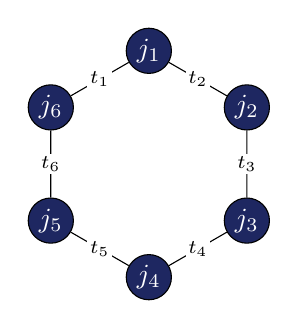
\begin{tikzpicture}[scale=1.15]
  \foreach \i in {1,...,6}{\node[draw,circle,fill=navy,text=white,inner sep=1.5pt]
    (j\i) at ({90-(\i-1)*60}:1.25) {$j_\i$};}
  \foreach \a/\b/\t in {1/2/2,2/3/3,3/4/4,4/5/5,5/6/6,6/1/1}{
    \draw (j\a)--(j\b) node[midway,fill=white,inner sep=1pt] {\scriptsize $t_\t$};}
\end{tikzpicture}

{\footnotesize $T_j=\{j,\,j{+}1 \bmod 6\}$, $b=3$}
\column{0.58\textwidth}
\begin{itemize}
  \item optimum: $\Zst=3$ --- a \emph{four}-group walk, one tool per transition
  \item heuristic ($\Kst=3$ groups, best order): $H=4$
\end{itemize}
\begin{alertblock}{gap $=1$, \quad ratio $=4/3$}
The grouping phase is to blame: minimal cardinality hides the cheaper
grouping. $g$ disjoint copies $\Rightarrow$ gap $=g$: \textbf{unbounded}.
\end{alertblock}
\end{columns}
\note{Costs free-initial (first magazine load not charged). Walk through: the
optimum keeps tool 1 resident; the heuristic must evict and reload it. This
instance recurs in every later result -- it is the fruit fly of the project.}
\end{frame}

\section{A worst-case theory of the heuristic}
\begin{frame}{The gap identified exactly}
\begin{theorem}[Grouping exactness]
$\displaystyle \Zst=\min_{\mathcal P}\gamma(\mathcal P)$ over \emph{all}
feasible groupings. Hence
$\;\mathrm{gap}=H-\Zst=$ the price of restricting to minimum cardinality.
\end{theorem}
\vspace{1mm}
Proved zero-gap classes (every $b$): \quad
$\Kst\le2$, \quad $|\U|\le b+1$, \quad $\Zst\le2$.
\end{frame}

\begin{frame}{The setup-cost spectrum: SSP $\longleftrightarrow$ JGP}
In practice a changeover costs a fixed setup $\rho$ beyond the per-tool swaps.
\begin{theorem}[Both ends explicit]
$\rho<\tfrac{1}{n-1}$ $\Rightarrow$ the augmented problem \emph{is} the SSP.\\
$\rho>H-\Zst$ $\Rightarrow$ every optimum uses minimum-cardinality grouping:
the heuristic is \emph{exactly optimal}.
\end{theorem}
\pause
\begin{itemize}
  \item the transition lives on $[\,1/(n-1),\ H-\Zst\,]$: it is governed by
        the \emph{gap itself};
  \item real tooling reports $\rho\approx3$--$60$ $\Rightarrow$ production
        sits far on the collapsed (JGP) side --- a rigorous licence for
        standard practice.
\end{itemize}
\note{Two messages. First, grouping is not an approximation device but an exact
lens; only the cardinality restriction costs. Second, the spectrum: both
thresholds explicit, transition governed by the gap itself; with realistic setup
costs the heuristic is provably optimal, answering the "real life" question of
how the SSP degenerates into the JGP.}
\end{frame}

\begin{frame}{The extremal law, quantitatively}
For $\Kst=3$ (configurations $\subseteq\U$, $q=|\U|-b$, $R=\Zst-q$):
\[
  H \;=\; q+\min\ \min\bigl(x_{ab},x_{bc},x_{ca}\bigr),
  \qquad x_{uv}=\bigl|(C_u\cap C_v)\setminus C_w\bigr|
\]
\[
  \mathrm{gap}\;\le\;\max\Bigl(0,\ \min\bigl(q,\ \bigl\lfloor\tfrac{2b-q}{3}\bigr\rfloor\bigr)-R\Bigr)
  \qquad\text{(tight at every known extremum)}
\]
\end{frame}

\begin{frame}{Bounds for every $\Kst$}
\[
  \frac{H}{\Zst}\;\le\;\min(b,\ \Kst-1,\ q)
\]
\pause
\[
  \mathrm{gap}\;\le\;\Bigl\lfloor\frac{q\,(b(\Kst-1)-q)}{b+q}\Bigr\rfloor - R
  \qquad\text{(random ordering of the groups + Jensen)}
\]
\pause
Zero-gap classes, every $b$: \quad $\Kst\le2$, \quad $|\U|\le b+1$,
\quad $\Zst\le2$.
\note{The exact H formula: choose the middle configuration to shield the overlap
of the outer two -- padding arguments eliminate configurations entirely. The
counting bound comes from double counting tool degrees over three
configurations; the general-K* bound from a random ordering of the groups plus
Jensen. Emphasise tightness: 6-ring, the b=4 witness and the b=5 witnesses all
attain the K*=3 bound exactly.}
\end{frame}

\begin{frame}{Determining the law: a certified elimination}
Natural candidate (all data $b\le4$): $\ \mathrm{gap}\le\Kst-2$.
\begin{itemize}
  \item \textbf{proved} for every $b\le4$ at $\Kst=3$, and outside the corner
        $2b\ge q+3R+6$ in general;
  \item the corner is nonempty --- and the law \textbf{fails} there:
\end{itemize}
\pause
\begin{alertblock}{Certificate ($b=5$, $\Kst=3$, $|\U|=9$)}
$T=(\{0,1,2,4,7\},\{0,4,5\},\{1,5\},\{2,6,8\},\{3,4,5,8\})$:\quad
$\Zst=4,\ H=6$ \\
gap $=2>\Kst-2$, ratio $3/2$ --- and it attains our quantitative bound
\emph{with equality}.
\end{alertblock}
\pause
Open (posed exactly): is
$\max\bigl(0,\min(q,\lfloor(2b-q)/3\rfloor)-R\bigr)$ the true worst case at
$\Kst=3$?\\[1mm]
{\footnotesize Status: attained at five $(b,q,R)$ points (two new, at $R=1$);
the $(5,3)$ and $(6,3)$ corners resist directed search --- the question lives
exactly there.}
\note{Frame as determination, not failure: the regime theorems said where the
candidate could fail; a directed search there produced the certificate in
minutes; the surviving quantitative law is tight at the very witness. This is
how extremal laws get pinned down. Prior evidence (1400 instances) was all
b<=4 -- exactly where the candidate is a theorem.}
\end{frame}

\begin{frame}{The $4/3$ ratio, and what remains}
\begin{theorem}[$b=3$]
Every instance with $\Kst\le3$ satisfies $H/\Zst\le 4/3$.
\end{theorem}
\begin{itemize}
  \item ingredients: gap $\le1$ at $\Kst=3,b=3$ (counting law) and
        positive gap $\Rightarrow \Zst\ge3$ (small-optimum lemma);
  \item the case $\Kst\ge4$ is the \emph{one} surviving conjecture ---
        populated (witnesses with ratio $5/4$ exist), no violation known;
  \item the edge-family pattern ``positive gap $\Rightarrow\Kst=3$'' does
        \emph{not} extend --- found and corrected this month.
\end{itemize}
\note{Honest status: 4/3 is now a theorem on most of its range and exactly one
regime remains conjectural. Mention the corrected assumption openly -- an
earlier draft leaned on the edge-family pattern; mixed-size instances broke it;
the proof route was repaired to not need it.}
\end{frame}

\section{Which structure decides the gap?}
\begin{frame}{Which structure decides these questions?}
\textbf{Negative (gap side).} Two instances with the \emph{same} circuit
clutter, same $\Kst$, same $\Zst$ have different gaps ($0$ vs $1$)
$\Rightarrow$ no job-compatibility invariant can decide exactness;
tool-level overlaps are essential.
\vspace{2mm}
\begin{theorem}[Covering side: odd rings, via blocking duality]
Clusters over maximal groups; blocker $=$ minimal covers ($\Kst=$ its min
size). On the $k$-ring, $b=3$: fractional cover $=k/2$, $\Kst=\lceil
k/2\rceil$ --- \textbf{tight iff $k$ even}.
\end{theorem}
Odd circular structure: first provable obstruction for the set-covering
relaxation behind JGP branch-and-price --- the parallel of odd holes.
\note{For Prof. Wagler: blocker = the dual clutter; the pair here is clusters
versus covers; Lehman transfers idealness between them. The hand computation:
weight one-half per adjacent pair. Question for the session: is odd-ring-like
structure the ONLY obstruction (an idealness characterisation)?}
\end{frame}

\section{The computational study}
\begin{frame}{The computational instrument}
\textbf{Why run it.} The theorems single out $|\U|-b$; the benchmark measures
it across the standard suites. And a prior question: the SSP's polynomial
loading subproblem is the textbook precondition for Benders --- untested until
now.
\vspace{1mm}
\begin{itemize}
  \item methods: 8 Benders configs (ours), LSS '04, Catanzaro-F4 '15,
        SSPMF '24, our branch-and-price (PCF$'$, PTF)
  \item 1{,}421 standard instances ($n\le40$, $|T|\le60$); 3600\,s / 600\,s;
        pinned threads; early stop after 8 straight failures
  \item one canonical metric: every returned sequence re-scored by KTNS
  \item integrity: $806$ instances solved by someone --- \textbf{zero}
        cross-method disagreements
\end{itemize}
\note{Stress the protocol choices: re-running baselines ourselves on one
machine/solver generation (cross-paper wall-clocks are meaningless); one
KTNS-based metric so objective conventions cannot distort; early-stop so weak
configurations do not burn weeks.}
\end{frame}

\begin{frame}{Results}
\begin{center}
\begin{tabular}{lcc}
\toprule
 & primary (411) & secondary (1{,}010)\\
\midrule
SSPMF (2024)            & \textbf{138}/165 & (not run, by design)\\
LSS (2004, modern CPLEX)& 91/98            & \textbf{668}/678\\
Catanzaro F4 (2015)     & 91/99            & 455/490\\
best Benders (ours)     & 1/9              & 26/48\\
PCF$'$ B\&P (ours, $n\le25$) & \multicolumn{2}{c}{94/379 pooled}\\
PTF B\&P (ours, $n\le25$)    & \multicolumn{2}{c}{72/351 pooled}\\
\bottomrule
\end{tabular}
\end{center}
\vspace{1mm}
\pause
\begin{itemize}
  \item SSPMF strongest on primary --- the published SOTA claim \emph{replicates}
  \item 2004 formulation $+$ modern solver $\approx$ 2015 formulation, and
        dominates secondary: solver generation outweighs formulation vintage
  \item everyone's wall: $n=15$ with $|T|\ge30$; nobody solves $n\ge30$
\end{itemize}
\note{Solved/attempted under early-stop; unattempted instances are at least as
hard as the last failures. The LSS observation is a benchmarking-hygiene point
for the community: comparisons against old formulations must state the solver
generation.}
\end{frame}

\begin{frame}{The diagnosis: bound-limited, mechanically}
Our Benders on capacity-loose instances: optimum found in seconds; the
\emph{proof} bound frozen at its trivial root value for the full hour
($\sim$250k nodes, $\sim$75k cuts). Fractional cuts: \textbf{structurally
inactive} --- no violated cut exists at fractional orderings (verified in
controlled runs).
\vspace{2mm}
\begin{block}{The measured split}
Among the $806$ solved instances: $\ 47.9\%$ have $\Zst=|\U|-b$ exactly
(upper-biased estimate). The suites split in half between the regime where
heuristic and exact methods win at the root, and the regime where new
mathematics is required.
\end{block}
PCF$'$/PTF confirm the same law from the branch-and-price side
($15\%$ of PCF$'$ optima at the root; PTF's stronger bound is the one lever
that exceeds $|\U|-b$).
\note{The frozen-bound mechanism: the master carries only pairwise information,
which vanishes at loose capacities -- our own theory's coverage row is the
one-line fix, implemented and queued as the fair re-test. The 48/52 split is
the report's thesis made empirical.}
\end{frame}

\section{Remaining work}
\begin{frame}{Programme}
\begin{enumerate}
  \item \textbf{Implemented, cluster re-run queued:} the Benders master with
        the coverage row $\theta\ge|\U|$ --- verified; on bound-tight
        instances the proof now closes \emph{at the root, with zero cuts}
        (the $6$-ring: $0$ cuts vs.\ $443$ before).
  \item \textbf{Theory (open):} the exact extremal law at $\Kst=3$
        (is the counting bound the truth?); the $4/3$ case $\Kst\ge4$.
  \item \textbf{With Prof.\ Wagler:} PTF polytope facets on the known
        witnesses (PORTA); the odd-ring idealness question for JGP.
\end{enumerate}
\vspace{2mm}
\emph{Questions for today:} which side of the blocking pair (clusters/covers
vs.\ circuits/groups) to pursue first; priority between the Benders re-run and
the polytope study; and whether the remaining theory items match your
expectations for the closing period.
\note{Close with ownership and three concrete questions. The coverage-row result is the freshest item: our own Proposition lb2, added as one master row, does what 443 Benders cuts could not on the ring -- say this plainly, it shows theory feeding back into the solver. Remaining risk is theory time only; nothing in the report depends on the open conjecture.}
\end{frame}

\end{document}
